\subsection{Region Transition Probability}

A travel path of a taxi can be simplified as a multi-hop process, in which a hop indicates an load/drop event happened. Seeing that, we define a \emph{ region transition probability} to figure out the probability of the next hop falling in a certain region $R_j$ from the current region $R_i$. Particularly, when two successive events are different: one load and one drop. Therefore, the region $R_i$ and $R_j$ are recognized by different metrics, that is, drop or load event distribution. For instance, if the taxi is currently occupied, then the next hop event is the drop one. Hence, choosing a target region from a region set obtained based on drop event distribution is more logical.

Before defining the region transition probability, we first describe our \textbf{region recognition process}.
Firstly, we divide the area into $100\times 100$ small grids, and define them as cells (as shown in the following equation) where $lon$ and $lat$ are relevant longitude and latitude, $len_x$ and $len_y$ are side length of the grid/cell).
\[C_{x,y}::=\{(lon,lat)|x \le \frac{{lon}}{{len_x}} < x + 1,
y \le \frac{{lat}}{{len_y}} < y + 1\}.\]
Then, we consider a region as a union of adjacent cells, as following.
\[R_m:: = \{ C_{x,y}|\exists C_{i,j} \in R_m
\Rightarrow \|x - i\| \le 1,\|y - j\| \le 1\}.\]
The main idea of clustering cells to regions is merging adjacent cells whose event density is larger than an event threshold $\eta$ into a same region.
For drop/load event, this process is conduct respectively. 
Three parameters, threshold $\eta$, Cluster Size and range $t$, are used in this process. 
Cluster Size defines the size of region, i.e., it is a limitation on the size of a region, saying $\|R_i\|\leq ClusterSize$.
We only consider the top $t$ regions, in which event density of each cells are larger than threshold $\eta$.
The overall clustering algorithm is shown as follows. We sort the $100 \times 100$ cells by event density in descending order, 
and begin with the first cell to search its neighbors whether to join the same region or not using breadth traversal. 
After the top t regions are formed, the other cells which do not belong to the top t regions will also be clustered into regions, 
whose size should still be small than Cluster Size. Consequently, every cells will be clustered into regions and the size of each region are not larger than Cluster Size.
By clustering cells into regions, two region sets, \textbf{$R^{load}$} and \textbf{$R^{drop}$}, can be recognized from the data set. As can be seen from Fig. \ref{figure_region_recognizition}, the differences among load region and drop regions for the Beijing taxi data set are clear.
In this figure, every colored block presents a region.In addition, Cluster Size = 200, range t = 200 (range is the same with Cluster Size by coincidence) and threshold $\eta = 121$ are set for load event and $\eta$ equates with 141 for drop event (these are set by the average event density of the top 5000 cells order by its event density).
\begin{figure}[!t]
\centering
\subfigure[drop event regions]{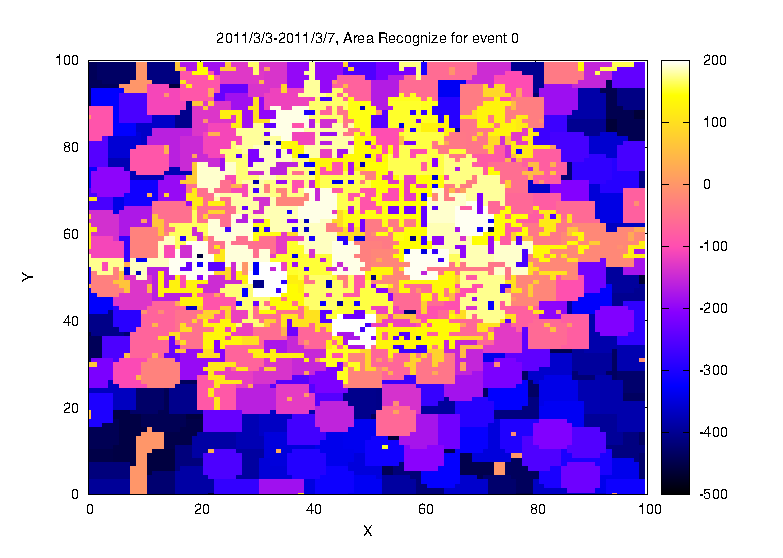
\includegraphics[width=0.23\textwidth]{figures_201103/region/Areas-2011_event0.eps}}
\subfigure[load event regions]{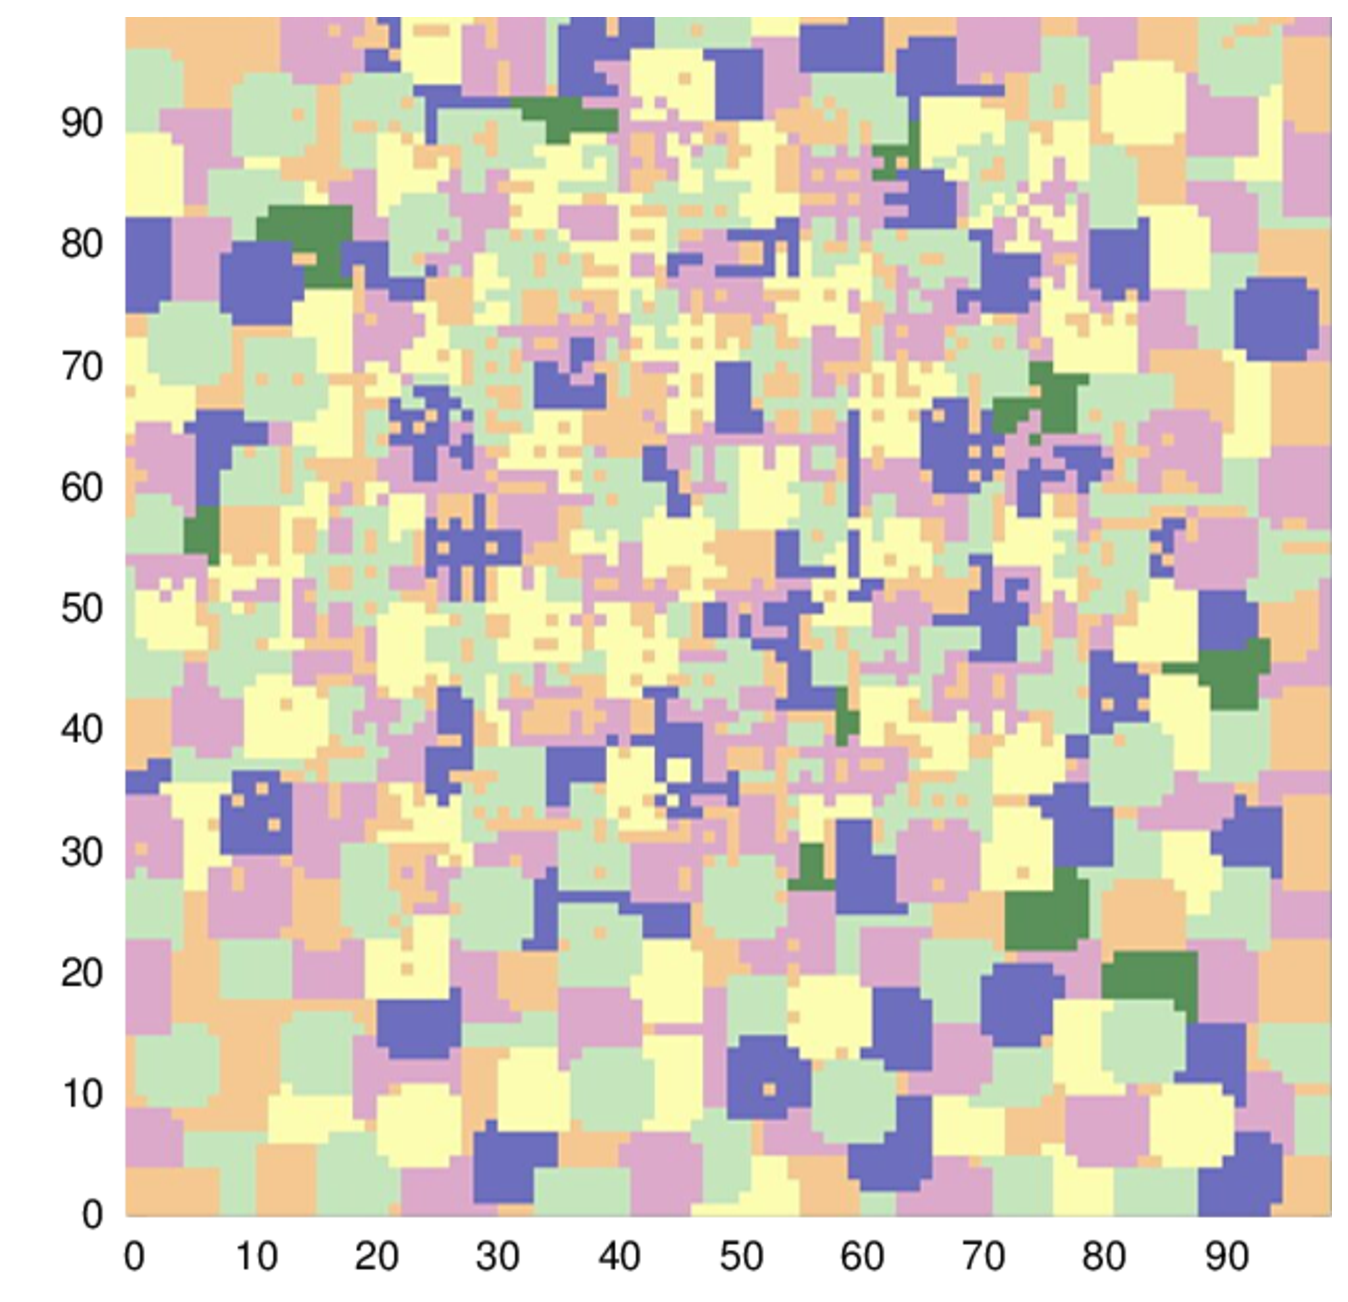
\includegraphics[width=0.23\textwidth]{figures_201103/region/Areas-2011_event1.eps}}
\centering
\caption{Region recognition}\label{figure_region_recognizition}
\end{figure}

\textbf{Calculation of region transition probability}: After clustering cells into regions, the transition probability from $R_i^{load}$ to $R_j^{drop}$ and the one from $R_i^{drop}$ to $R_j^{load}$, donated as $p_{i\rightarrow j}^{load\rightarrow drop}$ and $p_{i\rightarrow j}^{drop\rightarrow load}$, can be caculated. Since both transition probability can be calculated similarly, we only introduce the detailed one of $p_{i\rightarrow j}^{load\rightarrow drop}$.

First, we count all records in $R_i^{load}$ from the data set,  i.e. $REC_i^{load}=\{r~|~r.location\in{R_i^{load} \textit{ and }  r.event=load}\}$. Let $\|REC_i^{load}\|$ be the amount of such records. For record $r \in REC_i^{load}$, the next event and location can be easily obtained from the data set. Thus, we can get the set of such records whose next event is drop and next location is $R_j^{drop}$, i.e., $REC_{i\to j}^{load\to drop}=\{r~|~r.event=load,~r.event_{next}=drop,~r.location_{current}\in R_i^{load}, \textit{ and }  r.location_{next}\in R_j^{drop}\}$. Let $\|REC_{i\to j}^{load\to drop}\|$ be the amount of such records. We can then easily obtain the transition probability from $R_i^{load}$ to $R_j^{drop}$, as follows,
\[p_{i \to j}^{load \to drop} = \frac{\|REC_{i\to j}^{load\to drop}\|}{\|REC_i^{load}\|.}\]


\begin{table}
\caption{region recognization parameters}
\centering
\begin{tabular}{l|c|c|c|c}
  \hline
  Item & 0:00-8:59 &9:00-12:59&13:00-20:59 &21:00-23:59 \\
  \hline
  $\eta_{drop}$ & 556&84 &180 &51\\
  $\eta_{load}$ & 58&84 &182 &51\\
  $top$ & 200&200 &200 &200\\
  clusterSize& 500&500 &500 &500\\
  \hline
\end{tabular}
\end{table}